\documentclass[11pt, letterpaper]{report}
\usepackage[utf8]{inputenc}
\usepackage[T1]{fontenc}
\usepackage{helvet}
\renewcommand{\familydefault}{\sfdefault}
\usepackage{graphicx}
\usepackage{lipsum}
\usepackage[top=1in, bottom=1in, left=1in, right=1in]{geometry}
\usepackage{fancyhdr}
\usepackage{tocloft}
\usepackage{caption}
\captionsetup[figure]{labelfont={bf},name={Figure},labelsep=period, font={it}}
\usepackage{xltabular}

\usepackage{titlesec}
% Chapter formatting
\titleformat{\chapter}[hang] 
{\normalfont\huge\bfseries}{\thechapter}{1em}{} 
\titlespacing*{\chapter}{0pt}{0pt}{40pt}
% SubSection formatting
\titleformat{\subsection}
{\normalfont\large\bfseries}{}{0em}{}
\titlespacing*{\subsection}{0pt}{3.25ex plus 1ex minus .2ex}{1.5ex plus .2ex}
% SubSubSection formatting
\titleformat{\subsubsection}
{\normalfont\normalsize\bfseries}{\thesubsubsection}{1em}{}
\titlespacing*{\subsubsection}{0pt}{3.25ex plus 1ex minus .2ex}{1.5ex plus .2ex}

\author{Nishesh Jagga}

\begin{document}
% Cover page
\newgeometry{top=2in, bottom=2in, left=2in, right=2in}
\begin{titlepage}
    \centering
    
\includegraphics[width=\textwidth]{images/logo.png}\par
    \vspace{1cm}
    {\bfseries Software Requirements Specification\par}
    \vspace{5cm}
    {Group 01: \par}
    {Nishesh Jagga \par}
    {20741914 \par}
    {n2jagga \par}
\end{titlepage}
\restoregeometry

\tableofcontents
\clearpage

\listoffigures
\clearpage

% Section 1
\chapter{Introduction}
\setcounter{page}{1}

\section{Purpose}

\section{Scope}
A tool that aids a user in maintaining their budget by scheduling their weekly meals through suggesting recipes sourced from an online recipe database, that are suitable for their budget and align with their dietary restrictions. Following a personalization process, the users can expect to be presented with recipes that they might like to eat, made using ingredients that fit their budget, with prices from their local grocery store. To aid the grocery shopping process, any missing ingredients for the recipes in their planned meals would be added to a grocery list for the user to follow while shopping.

\section{Definitions, Acronyms, and Abbreviations}

\section{References}

% Section 2
\chapter{Overall Description}

\section{Product Perspective}

\section{Product Functions}

\subsection{Use Case Model}
\begin{figure}[h]
    \centering
    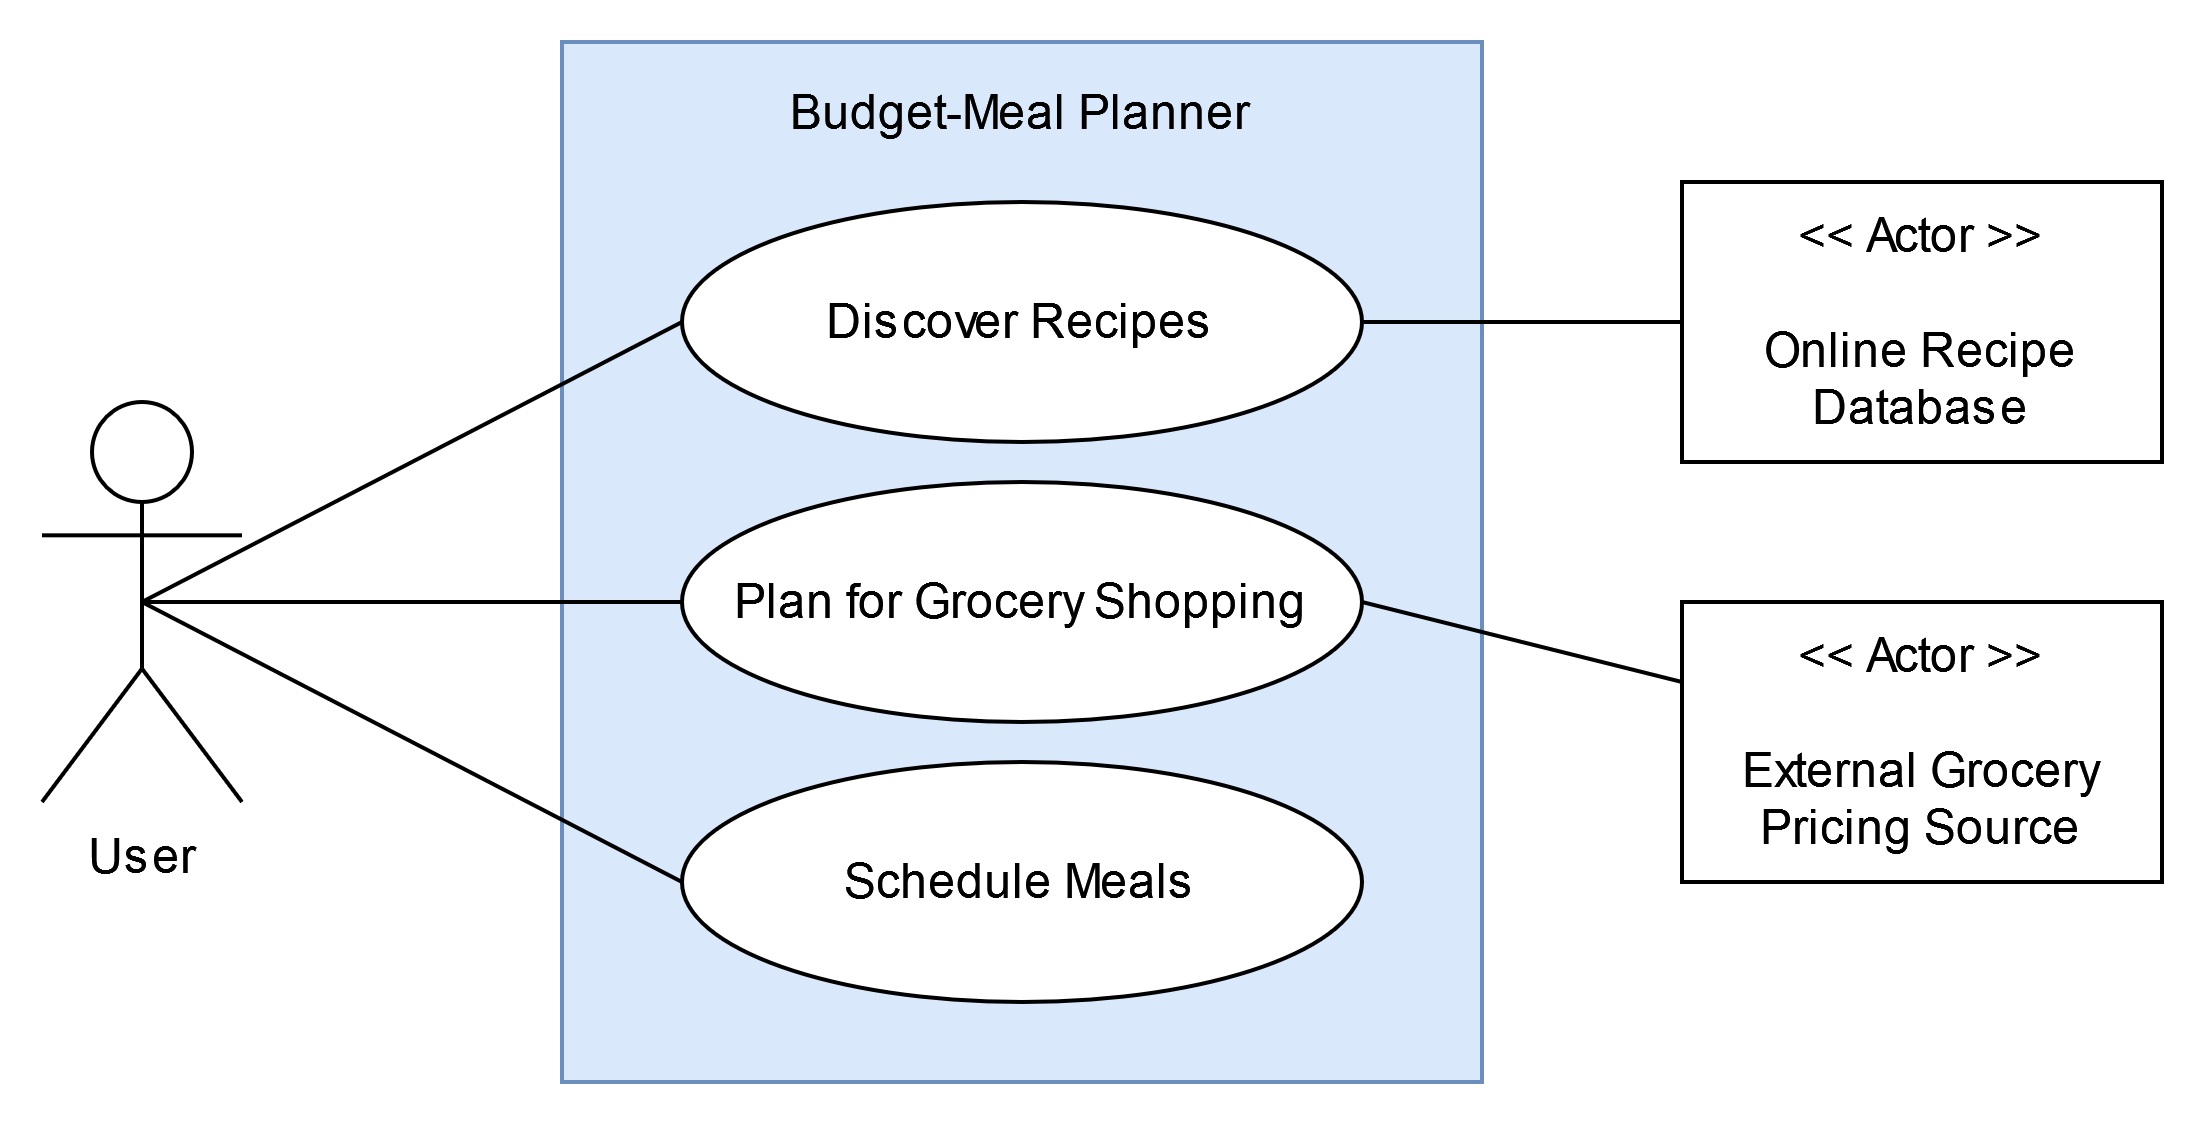
\includegraphics[width=\textwidth]{images/Use_Case.png}
    \caption{Use Case Model}
\end{figure}

\section{Discover Recipes}
\begin{itemize}
    \item Accept the users’ login credentials and open their account.
    \item Ask the user some questions to gather their preferences.
    \item Present the user with a list of recipes recommended for them.
    \item Accept a new recipe from the user and save it.
    \item Suggest alternative recipes, similar to the current recipe displayed.
    \item Hide a recipe from the user if they dislike it.
    \item Save a recipe to a “liked” collection for the user if they like it.
\end{itemize}
\textbf{Domain Assumptions}
\begin{itemize}
    \item The user has an account.
    \item Online Recipe Database is available.
    \item External Grocery Pricing Source is available.
    \item Recipe is valid, and can be cooked.
    \item The ingredients in the recipe are available in the External Grocery Pricing Source or the user’s pantry.
\end{itemize}

\section{Plan for Grocery Shopping}
\begin{itemize}
    \item Display the user’s current ingredient quantities in the pantry.
    \item Display the user’s grocery list.
    \item Add all ingredients from a recipe to the grocery list.
    \item Move ingredients from grocery list to pantry based on what the user bought from the grocery store.
\end{itemize}
\textbf{Domain Assumptions}
\begin{itemize}
    \item The user has an account.
    \item External Grocery Pricing Source is available.
    \item The currency of the External Grocery Pricing Source is the same as the user’s currency.
    \item The prices are up to date, and representative of the real world.
\end{itemize}

\section{Schedule Meals}
\begin{itemize}
    \item Assign a recipe to a meal on a user’s schedule.
    \item Display a user’s meal plan (schedule).
\end{itemize}
\textbf{Domain Assumptions}
\begin{itemize}
    \item The user has an account.
    \item Recipes are accessible.
    \item There are enough recipes available to fill the user’s schedule.
    \item The ingredients for the meals are available in the user’s pantry, or can be procured.
\end{itemize}

\section{User Characteristics}

\section{Assumptions and Dependencies}

% Section 3
\chapter{Specific Requirements}

\section{Domain Model}
Describe the domain model here!!

\begin{figure}[h]
    \centering
    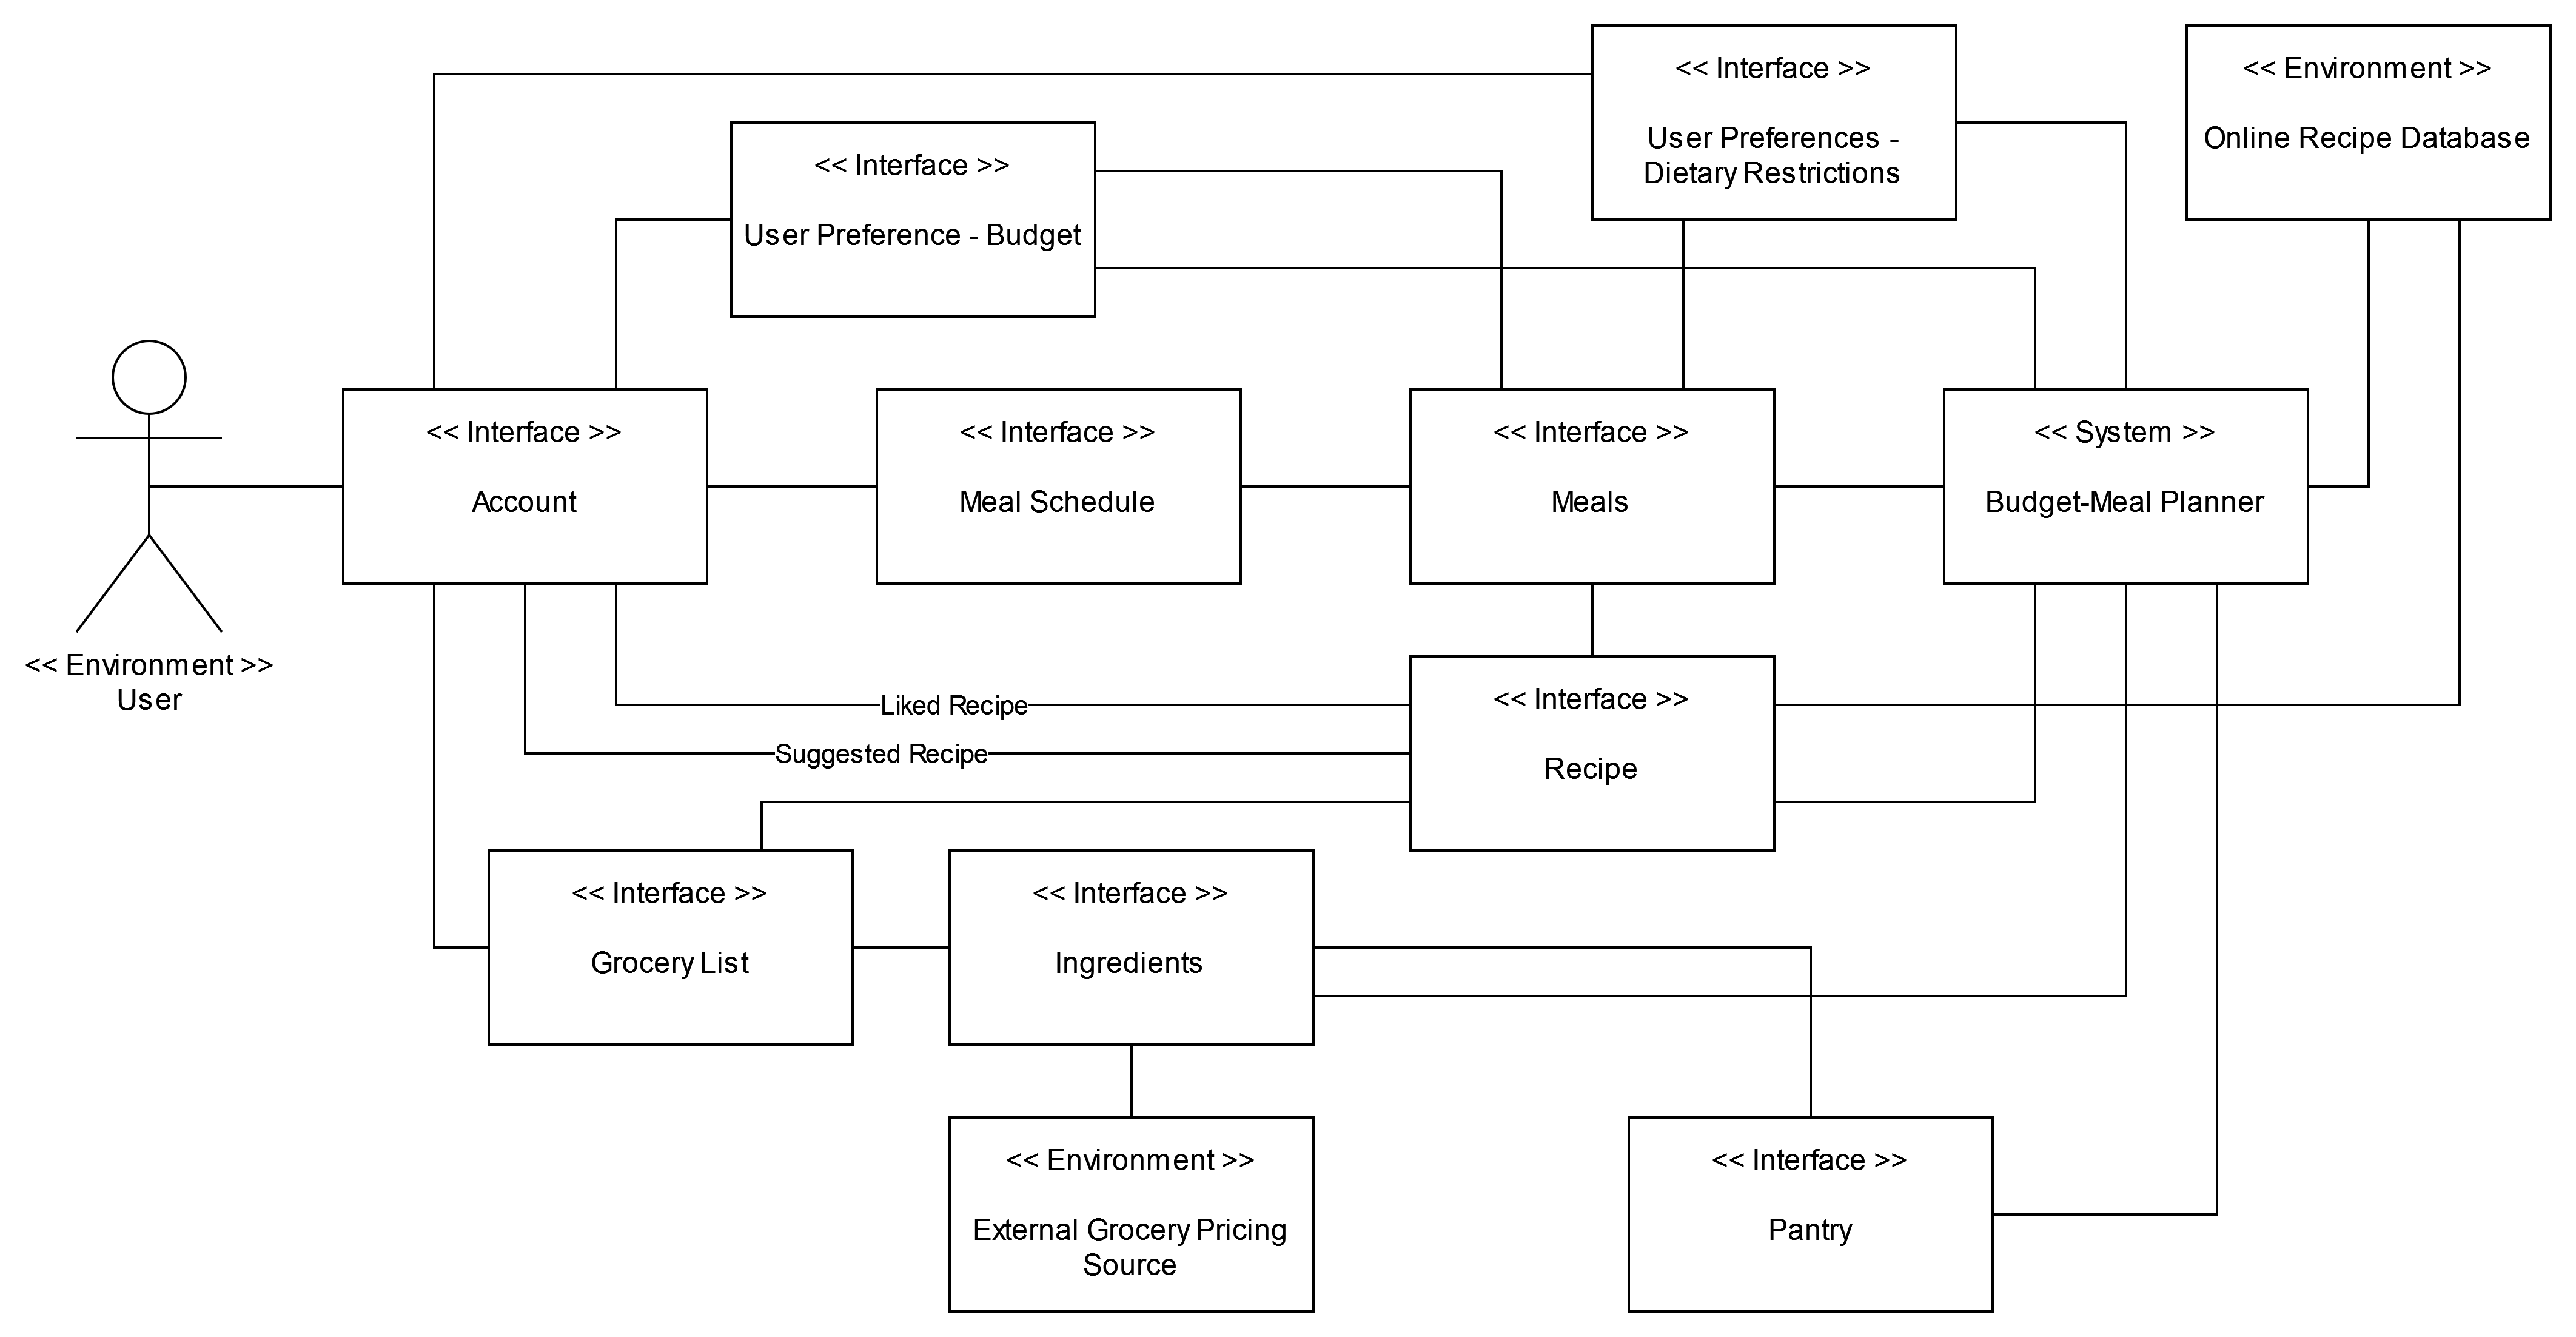
\includegraphics[width=\textwidth]{images/Domain_Model.png}
    \caption{Domain Model with World Diagram Superimposed}
\end{figure}


\section{Scenarios}
\subsection{UC 1: Discover Recipes}
% START UC 1 TABLES

\begin{xltabular}{\textwidth}{|X|X|X|}
\hline
User & Budget-Meal Planner & Online Recipe Database \\
\hline
1. Opens the Budget-Meal Planner &  &  \\
 & 2. Displays the login screen &  \\
3. Types in their username and password &  &  \\
 & 4. The user is logged in to the account with matching credentials &  \\
 & 5. The "Home" screen is displayed &  \\
6. Clicks the "Discover Recipes" button &  &  \\
 & 7. Displays a page with a search box at the top and a scrollable collection of the top 15 recipes related to the user's preferences, which have not been saved by the user &  \\
8. Clicks on a recipe &  &  \\
 & 9. Displays the recipe's details &  \\
10. Clicks the "Like" button &  &  \\
 & 11. Saves the recipe to the user's account, in the "Liked Recipes" section &  \\
12. Clicks the "Back" button &  &  \\
 & 13. Displays the collection of recipes again &  \\
14. Clicks the search box &  &  \\
 & 15. Displays a search bar with a "Search" button &  \\
16. Types in a search query &  &  \\
 & 17. Forwards the search query to the Online Recipe Database &  \\
 &  & 18. Returns a collection of recipes related to the search query \\
 & 19. Compares the collection of recipes returned by the online recipe database with the collection of recipes already saved to the user's account &  \\
 & 20. Removes any recipes already saved to the user's account from the collection and displays the remaining collection of recipes &  \\
21. Go To 8 &  &  \\
22. Clicks the "Home" button to return to the Home page &  &  \\
\hline
\end{xltabular}

\begin{xltabular}{\textwidth}{|X|X|X|}
\hline
\multicolumn{3}{|p{\dimexpr\linewidth-2\tabcolsep\relax}|}{Exception 1: The user enters an incorrect username or password} \\
\hline
User & Budget-Meal Planner & Online Recipe Database \\
\hline
 & E1.4. Checks the database for a matching username, if user does not exist, displays an error message, "Incorrect username or password. Try again." &  \\
E1.5. Go To 3 &  &  \\
 &  &  \\
\hline
\end{xltabular}

\begin{xltabular}{\textwidth}{|X|X|X|}
\hline
\multicolumn{3}{|p{\dimexpr\linewidth-2\tabcolsep\relax}|}{Exception 2: The online recipe database is unavailable} \\
\hline
User & Budget-Meal Planner & Online Recipe Database \\
\hline
 & E2.18. Attempts to connect to the online recipe database source &  \\
 &  & E2.19. No response or connection refused \\
 & E2.20. Retries the connection 3 times &  \\
 &  & E2.21. No response or connection refused after 3 retries \\
 & E2.22. Displays an error message, "Unable to retrieve search results. Please try again later." &  \\
E2.23. Acknowledges the error message &  &  \\
 & E2.24. Go To 7 &  \\
 &  &  \\
\hline
\end{xltabular}
% END UC 1 TABLES

\subsection{UC 2: Plan for Grocery Shopping}
% START UC 2 TABLES

\begin{xltabular}{\textwidth}{|X|X|X|}
\hline
User & Budget-Meal Planner & External Grocery Pricing Source \\
\hline
1. Clicks the "Grocery List" button &  &  \\
 & 2. Displays the user's empty grocery list with the message, "Add something to the list!", and a button to add ingredients &  \\
3. Clicks the "Add ingredients" button &  &  \\
 & 4. Displays a search bar and a list of common ingredients &  \\
5. Types in the search bar &  &  \\
 & 6. Displays a list of ingredients matching the search query &  \\
7. Clicks on an ingredient &  &  \\
 & 8. Displays a prompt, "How much {ingredient name} do you want to add?" and a number input field, along with the options "Yes" and "No" &  \\
9. Enters the quantity of the ingredient to add to the grocery list &  &  \\
 & 10. Updates the number input field with the quantity entered by the user &  \\
11. Clicks the "Yes" button &  &  \\
 & 12. Returns to the grocery list, with the ingredient added to the list with the quantity entered by the user &  \\
 & 13. Requests for the latest prices of ingredients in the grocery list from the external grocery pricing source. Rate limited to once per day. &  \\
 &  & 14. Returns the latest prices of ingredients in the grocery list \\
 & 15. Displays the user's grocery list with the latest prices &  \\
16. Clicks the checkbox next to the ingredient &  &  \\
 & 17. Displays a confirmation message, "Add ingredient to pantry?" with the options "Yes", "No", and "Modify Quantity" &  \\
18. Clicks the "Yes" button &  &  \\
 & 19. Moves the ingredient to the pantry, adds the quantity in the grocery list to what was already in the pantry &  \\
 & 20. Displays the user's pantry, containing a scrollable list of ingredients and their quantities &  \\
21. Clicks the "Home" button to return to the Home page &  &  \\
\hline
\end{xltabular}

\begin{xltabular}{\textwidth}{|X|X|X|}
\hline
\multicolumn{3}{|p{\dimexpr\linewidth-2\tabcolsep\relax}|}{Exception 1: The user's search query does not match any ingredients} \\
\hline
User & Budget-Meal Planner & External Grocery Pricing Source \\
\hline
 & E1.6. Displays a message, "No results found..." &  \\
E1.7. Go To 5 &  &  \\
 &  &  \\
\hline
\end{xltabular}

\begin{xltabular}{\textwidth}{|X|X|X|}
\hline
\multicolumn{3}{|p{\dimexpr\linewidth-2\tabcolsep\relax}|}{Exception 2: The external grocery pricing source is unavailable} \\
\hline
User & Budget-Meal Planner & External Grocery Pricing Source \\
\hline
 & E2.14. Attempts to connect to the external grocery pricing source &  \\
 &  & E2.15. No response or connection refused \\
 & E2.16. Retries the connection 3 times &  \\
 &  & E2.17. No response or connection refused after 3 retries \\
 & E2.18. Displays an error message, "Unable to retrieve latest prices. Please try again later." &  \\
E2.19. Acknowledges the error message &  &  \\
 & E2.20. Displays the user's grocery list with the latest prices from the last successful request &  \\
E2.21. Go To 5 &  &  \\
 &  &  \\
\hline
\end{xltabular}
% END UC 2 TABLES

\subsection{UC 3: Schedule Meals}
% START UC 3 TABLES

\begin{xltabular}{\textwidth}{|X|X|}
\hline
User & Budget-Meal Planner \\
\hline
1. Clicks the "Schedule" button &  \\
 & 2. Prompts the user with a message, "Schedule meals for the week?" \\
3. Clicks the "Yes" button &  \\
 & 4. Selects recipes from the app's local recipe database, and assigns them to every meal slot for the week \\
 & 5. Displays the user's weekly meal plan schedule \\
6. Clicks on a day of the week &  \\
 & 7. Displays the user's meal plan for that day \\
8. Clicks on a time slot for a meal &  \\
 & 9. Displays the meal details page \\
10. Clicks on a recipe &  \\
 & 11. Displays the recipe's details \\
12. Clicks the "Add ingredients to Grocery List" button &  \\
 & 13. Displays a confirmation message, "Add all ingredients to Grocery List?" with the options "Yes" and "No" \\
14. Clicks the "Yes" button &  \\
 & 15. Adds all ingredients in the recipe to the user's grocery list, adding quantities wherever possible \\
16. Clicks the "Home" button to return to the Home page &  \\
\hline
\end{xltabular}

\begin{xltabular}{\textwidth}{|X|X|}
\hline
\multicolumn{2}{|p{\dimexpr\linewidth-2\tabcolsep\relax}|}{Exception 1: The app is unable to find recipes for a meal slot} \\
\hline
User & Budget-Meal Planner \\
\hline
 & E1.4. Displays an error message, "Unable to find recipes to schedule. Please try again later." \\
E1.5. Acknowledges the error message &  \\
 & E1.6. Go To UC1.5 \\
 &  \\
\hline
\end{xltabular}

\begin{xltabular}{\textwidth}{|X|X|}
\hline
\multicolumn{2}{|p{\dimexpr\linewidth-2\tabcolsep\relax}|}{Exception 2: Fails to add ingredients to grocery list} \\
\hline
User & Budget-Meal Planner \\
\hline
 & E2.14. Displays an error message, "Unable to add ingredients to grocery list. Please try again." \\
E2.15. Acknowledges the error message &  \\
 & E2.16. Go To 11 \\
 &  \\
\hline
\end{xltabular}
% END UC 3 TABLES

% User Stories
\section{User Stories}

\subsection{Discover Recipes}

\subsubsection{User Story 1}
As a user, I want to be able to login so that I can access my personalized recipe recommendations.

\subsubsection{Test Case 1.1}
Check if the user can enter their login credentials.

\subsubsection{Test Case 1.2}
Check if the user can access their account after providing valid credentials.

\subsubsection{User Story 2}
As a user, I want to receive personalized recipe recommendations so that I can discover new recipes that align with my preferences.

\subsubsection{Test Case 2.1}
Check if the user receives recipe recommendations based on their preferences after logging in.

\subsubsection{Test Case 2.2}
Check if the recipe recommendations update when the user's preferences change.

\subsubsection{User Story 3}
As a user, I want to be able to add new recipes so that I can expand my collection of potential meals.

\subsubsection{Test Case 3.1}
Check if the user can add a new recipe.

\subsubsection{Test Case 3.2}
Check if the added recipe appears in the user's recipe list.

\subsubsection{User Story 4}
As a user, I want to be able to hide recipes I dislike so that they don't appear in my future recommendations.

\subsubsection{Test Case 4.1}
Check if the user can hide a recipe.

\subsubsection{Test Case 4.2}
Check if the hidden recipe no longer appears in the recommendation list.

\subsubsection{User Story 5}
As a user, I want to be able to save recipes I like so that I can easily find them later.

\subsubsection{Test Case 5.1}
Check if the user can save a recipe.

\subsubsection{Test Case 5.2}
Check if the saved recipe appears in the user's saved recipes list.

\subsubsection{User Story 6}
As a user, I want to be able to view the details of a recipe so that I can learn how to prepare it.

\subsubsection{Test Case 6.1}
Check if the user can view the details of a recipe.

\subsubsection{User Story 7}
As a user, I want to be able to search for specific recipes so that I can find something specific I want to cook.

\subsubsection{Test Case 7.1}
Check if the user can search for a specific recipe.

\subsubsection{Test Case 7.2}
Check if the search results are relevant to the search query.

\subsubsection{User Story 8}
As a user, I want to be able to view my liked recipes so I can refer back to them whenever I want.

\subsubsection{Test Case 8.1}
Check if the user can access their list of liked recipes.

\subsubsection{User Story 9}
As a user, I want to be able to remove recipes from my liked list so I can manage the recipes I'm interested in.

\subsubsection{Test Case 9.1}
Check if the user can remove a recipe from their liked list.

\subsection{Plan for Grocery Shopping}

\subsubsection{User Story 10}
As a user, I want to be able to view my grocery list so that I know what I need to buy.

\subsubsection{Test Case 10.1}
Check if the user can view their grocery list.

\subsubsection{User Story 11}
As a user, I want to be able to add ingredients to my grocery list so that I can remember to buy them.

\subsubsection{Test Case 11.1}
Check if the user can add ingredients to their grocery list.

\subsubsection{User Story 12}
As a user, I want to be able to remove ingredients from my grocery list so that I can keep the list updated.

\subsubsection{Test Case 12.1}
Check if the user can remove ingredients from their grocery list.

\subsubsection{User Story 13}
As a user, I want to be able to see the latest prices of the ingredients in my grocery list so that I can budget for my shopping.

\subsubsection{Test Case 13.1}
Check if the user can view the latest prices of the ingredients in the grocery list.

\subsubsection{User Story 14}
As a user, I want to be able to update the quantities of ingredients in my pantry after cooking so that my pantry list remains accurate.

\subsubsection{Test Case 14.1}
Check if the user can update the quantities of ingredients in their pantry.

\subsubsection{User Story 15}
As a user, I want to be able to add all ingredients from a recipe to my grocery list so that I can ensure I have everything I need to cook the meal.

\subsubsection{Test Case 15.1}
Check if the user can add all ingredients from a recipe to the grocery list.

\subsubsection{User Story 16}
As a user, I want to be able to move ingredients from my grocery list to my pantry so that I can keep track of what I have bought.

\subsubsection{Test Case 16.1}
Check if the user can move ingredients from the grocery list to the pantry.

\subsubsection{Test Case 16.2}
Check if the moved ingredient is removed from the grocery list and added to the pantry.

\subsubsection{User Story 17}
As a user, I want to be able to modify the quantities of ingredients in my grocery list so that I can adjust based on my needs.

\subsubsection{Test Case 17.1}
Check if the user can modify the quantities of ingredients in the grocery list.

\subsubsection{User Story 18}
As a user, I want to be able to view the current quantities of ingredients in my pantry so that I know what I have on hand.

\subsubsection{Test Case 18.1}
Check if the user can view the current quantities of ingredients in the pantry.

\subsection{Schedule Meals}

\subsubsection{User Story 19}
As a user, I want to be able to create a meal plan so that I can organize my meals for the week.

\subsubsection{Test Case 19.1}
Check if the user can create a meal plan for the week.

\subsubsection{User Story 10}
As a user, I want to be able to view my meal plan so that I can see what I have planned to eat.

\subsubsection{Test Case 20.1}
Check if the user can view their meal plan.

\subsubsection{User Story 21}
As a user, I want to be able to assign a recipe to a meal on my schedule so that I can plan when to cook and eat each meal.

\subsubsection{Test Case 21.1}
Check if the user can assign a recipe to a meal on their schedule.

\subsubsection{User Story 22}
As a user, I want to be able to view the details of a meal in my schedule so that I can see what I need to prepare.

\subsubsection{Test Case 22.1}
Check if the user can view the details of a meal in their schedule.

\subsubsection{User Story 23}
As a user, I want to be able to add all ingredients from a recipe in my meal plan to my grocery list so that I can make sure I have everything I need.

\subsubsection{Test Case 23.1}
Check if the user can add all ingredients from a recipe in their meal plan to their grocery list.

\subsubsection{User Story 24}
As a user, I want to be able to modify my meal plan so that I can adjust based on changes in my schedule or preferences.

\subsubsection{Test Case 24.1}
Check if the user can modify their meal plan.

\subsubsection{User Story 25}
As a user, I want to be able to remove meals from my meal plan so I can adjust my plan when necessary.

\subsubsection{Test Case 25.1}
Check if the user can remove meals from their meal plan.

\end{document}
